
\documentclass{article}
\usepackage[utf8]{inputenc}
\usepackage[T1]{fontenc}
\usepackage{lmodern}
\usepackage{amsmath, amssymb, amsfonts, amsthm, stmaryrd}
\usepackage{tikz}
\usetikzlibrary{matrix,arrows}
\usepackage{tikz-cd}
\usepackage{geometry}
\usepackage[french]{babel}
\usepackage{amsopn}
\usepackage{dsfont}
\usepackage{booktabs}
\usepackage{graphicx}

% indicatrice : \mathbb{1} pioche un glyphe de msbm qui n'est pas une vraie
% double barre ; \mathds{1} (dsfont) oui. Repli sans dsfont : \mathbf{1}
\newcommand{\ind}{\mathds{1}}

\theoremstyle{remark}
\newtheorem{remarque}{Remarque}

\title{Une méthode solide de test statistique pour détecter les manoeuvres}
\author{Etienne Chevrolat}
\date{}

\begin{document}

\maketitle

\begin{abstract}
    On cherche ici à expliquer une méthode statistique avancée pour tester la présence de ruptures au sein des séries de paramètres orbitaux.
    On teste à la fois des ruptures de niveau (manoeuvres impulsionnelles), et des ruptures de pentes (manoeuvres type propulsion électrique).
\end{abstract}

\section{Le modèle statistique}

\subsection*{Le cadre}

On va considérer $y_{\mathrm{sat}}$ un paramètre orbital issu d'un TLE (demi-grand axe ou inclinaison par exemple) sur un historique long (2000 TLEs par exemple).

On découpe cet historique long en fenêtres courtes de $N = 24$ TLEs, la taille retenue
dans le code. 

Considérons donc une de ces fenêtres. On réindexe le temps sur le milieu de la fenêtre :
\[
\tau_k = t_k - t_{\mathrm{centre}}, \qquad k = 1, \dots, N .
\]
L'instant central $t_{\mathrm{centre}}$ est l'instant où a lieu la manoeuvre s'il y en a une dans cette fenêtre temporelle.

Sur cette fenêtre temporelle courte, on va approximer $y_{\mathrm{sat}}$ par son polynôme de Taylor à l'ordre $p$ ainsi que par des termes de ruptures :

\[
y_{\mathrm{sat}}(\tau) = c_0 + c_1 \tau ^1 + \cdots + c_p \tau ^ p + A_{\mathrm{niveau}} \ind_{\tau > 0} + B_{\mathrm{pente}} \max(0, \tau) + \varepsilon 
\]

\begin{figure}[htbp]
\centering
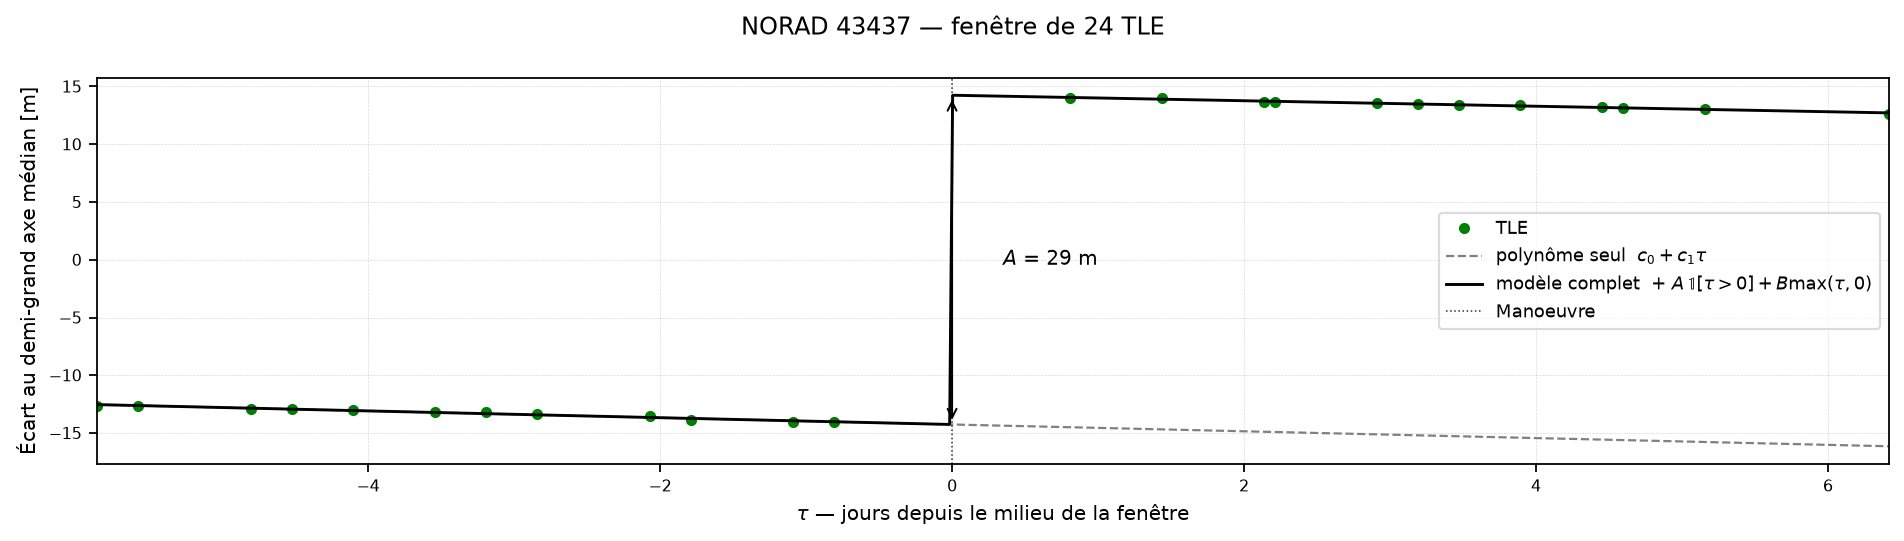
\includegraphics[width=\textwidth]{figures/stat_modele.png}
\end{figure}

\begin{center}
\fbox{%
\begin{minipage}{0.9\textwidth}
\textbf{Modèle linéaire gaussien}

\medskip
On considère un bruit gaussien $\varepsilon \sim \mathcal{N}(0, \sigma^2 I_N)$. On peut alors
réécrire l'approximation précédente sous la forme
$y_{\mathrm{sat}} = X\beta + \varepsilon$, avec
\[
X = \begin{pmatrix}
1 & \cdots & \tau_1^p & \ind_{\tau_1 > 0} & \max(0, \tau_1) \\
1 & \cdots & \tau_2^p & \ind_{\tau_2 > 0} & \max(0, \tau_2) \\
\vdots & \ddots & \vdots & \vdots & \vdots \\
1 & \cdots & \tau_N^p & \ind_{\tau_N > 0} & \max(0, \tau_N)
\end{pmatrix}
\qquad \text{et} \qquad
\beta = \begin{pmatrix}
c_0 \\ c_1 \\ \vdots \\ c_p \\ A_{\mathrm{niveau}} \\ B_{\mathrm{pente}}
\end{pmatrix}
\]
\end{minipage}}
\end{center}

\subsection*{Approximation des paramètres}
A partir des mesures effectives de $y_{\mathrm{sat}}$, on peut estimer les paramètres $\beta$ par la méthode du maximum de vraisemblance. Cela revient à résoudre le problème d'optimisation suivant :
\[
\hat{\beta} = \operatorname*{arg\,max}_{\beta} \log p(y_{\mathrm{sat}} \mid X, \beta)
\]
Le bruit étant gaussien, la vraisemblance s'écrit explicitement
\[
p(y_{\mathrm{sat}} \mid X, \beta) = (2\pi\sigma^2)^{-N/2} \exp\left( -\frac{\lVert y_{\mathrm{sat}} - X\beta \rVert^2}{2\sigma^2} \right),
\]
donc
\[
\log p(y_{\mathrm{sat}} \mid X, \beta) = -\frac{N}{2}\log(2\pi\sigma^2) - \frac{1}{2\sigma^2} \lVert y_{\mathrm{sat}} - X\beta \rVert^2 .
\]
D'où :
\[
\hat{\beta} = \operatorname*{arg\,max}_{\beta} \log p(y_{\mathrm{sat}} \mid X, \beta) = \operatorname*{arg\,min}_{\beta} \lVert y_{\mathrm{sat}} - X\beta \rVert^2 .
\]
\emph{Sous modèle gaussien, maximum de vraisemblance équivaut aux moindres carrés}.

La fonction $\beta \mapsto \lVert y_{\mathrm{sat}} - X\beta \rVert^2$ est convexe et différentiable, de
gradient $-2X^{\top}(y_{\mathrm{sat}} - X\beta)$. On obtient : 
\[
X^{\top}X \hat{\beta} = X^{\top} y_{\mathrm{sat}} .
\]
On suppose désormais que $X$ est de rang maximal, $\operatorname{rang}(X) = q$ où l'on note
\[
q := p + 3 \quad \text{(nombre de paramètres)}, \qquad \nu := N - q \quad \text{(degrés de liberté résiduels)} .
\]
Sous cette hypothèse $X^{\top}X$ est inversible, d'où
\[
\boxed{\ \hat{\beta} = (X^{\top}X)^{-1} X^{\top} y_{\mathrm{sat}} \ }
\]

\subsection*{Résidus et estimation du bruit}

Introduisons le projecteur orthogonal sur l'espace engendré par les colonnes de $X$, et son
complément :
\[
P = X(X^{\top}X)^{-1}X^{\top}, \qquad M = I_N - P .
\]
Ce sont des matrices symétriques et idempotentes, de rangs respectifs $q = p+3$ et $\nu$. 
Le vecteur des résidus s'écrit alors
\[
r = y_{\mathrm{sat}} - X\hat{\beta} = M y_{\mathrm{sat}} = M(X\beta + \varepsilon) = M\varepsilon ,
\]
donc les résidus ne dépendent que du bruit, jamais de la valeur des paramètres. 
L'estimateur débiaisé du bruit est : 
\[
\hat{\sigma}^2 = \frac{\lVert r \rVert^2}{N - q} = \frac{\lVert y_{\mathrm{sat}} - X\hat{\beta} \rVert^2}{\nu} .
\]

Sous les hypothèses précédentes :
\begin{enumerate}
    \item $\hat{\beta} \sim \mathcal{N}\left( \beta, \ \sigma^2 (X^{\top}X)^{-1} \right)$ ;
    \item $\dfrac{\nu \hat{\sigma}^2}{\sigma^2} \sim \chi^2_{\nu}$ ;
    \item $\hat{\beta}$ et $\hat{\sigma}^2$ sont indépendants.
\end{enumerate}

\section{Le test de rupture de niveau}

\subsection*{L'hypothèse nulle}

Détecter une manoeuvre impulsionnelle en $t_{\mathrm{centre}}$, c'est décider si le coefficient de
rupture de niveau est significativement non nul. C'est le coefficient $A_{niveau}$ en position $p+2$ de $\beta$.
On teste
\[
\mathcal{H}_0 : A = 0
\qquad \text{contre} \qquad
\mathcal{H}_1 : A \neq 0 .
\]
Le test est \emph{bilatéral} : une manoeuvre peut aussi bien monter que baisser le demi-grand
axe.

Posons
\[
v_A := \left[ (X^{\top}X)^{-1} \right]_{p+2,\,p+2}.
\]

\subsection*{La statistique de test suit une loi de Student}

Sous les hypothèses du modèle et sous $\mathcal{H}_0$, la statistique
\[
\boxed{\ T = \frac{\hat{A}}{\hat{\sigma} \sqrt{v_A}} \ }
\]
suit une loi de Student à $\nu = N - q$ degrés de liberté.

\begin{figure}[htbp]
\centering
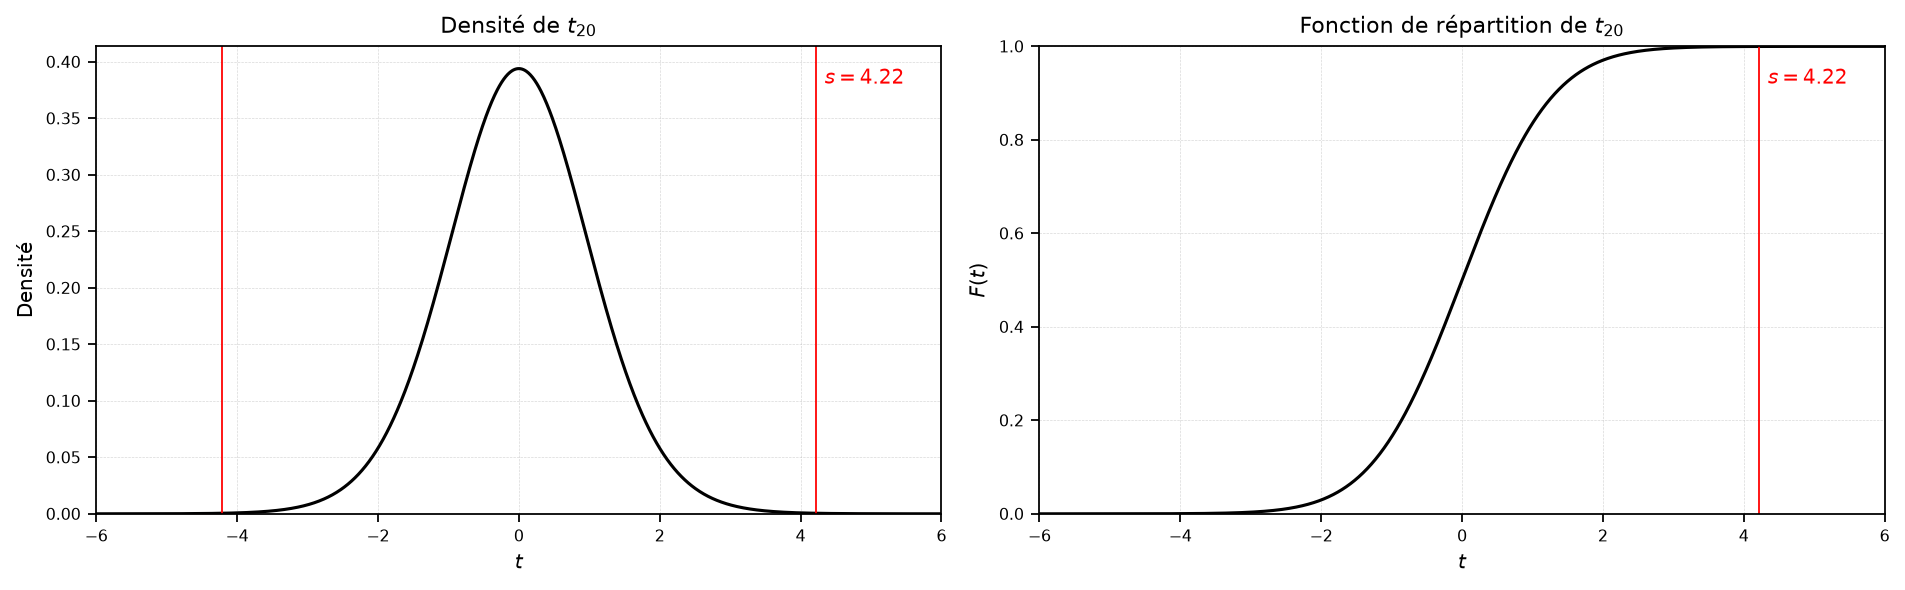
\includegraphics[width=\textwidth]{figures/stat_student.png}
\end{figure}

\begin{remarque}
Sous $\mathcal{H}_1$, le même calcul montre que $T$ suit une loi de Student \emph{décentrée} de
paramètre
\[
\delta = \frac{A}{\sigma \sqrt{v_A}} .
\]
C'est ce $\delta$, qui gouverne la détectabilité : une manoeuvre se voit si son
amplitude est grande devant le bruit et ramené à la géométrie de la fenêtre par $\sqrt{v_A}$.
\end{remarque}

\subsection*{Règle de décision et p-valeur}

Soit $F$ la fonction de répartition de la loi $T$. La p-valeur associée à une valeur
observée $T_{\mathrm{obs}}$ est la probabilité, sous $\mathcal{H}_0$, d'observer un écart au moins aussi
extrême :
\[
p = \mathbb{P}_{\mathcal{H}_0}\left( |T| \geq |T_{\mathrm{obs}}| \right) = 2\left( 1 - F(|T_{\mathrm{obs}}|) \right) .
\]
On rejette $\mathcal{H}_0$, c'est-à-dire on déclare une manoeuvre, au niveau $\alpha$ lorsque
\[
p < \alpha
\qquad \Longleftrightarrow \qquad
|T_{\mathrm{obs}}| > s_{\alpha} := F^{-1}\left( 1 - \tfrac{\alpha}{2} \right) .
\]
Par construction $\mathbb{P}_{\mathcal{H}_0}(|T| > s_{\alpha}) = \alpha$ exactement : $\alpha$
est la probabilité de crier à la manoeuvre \emph{sur une fenêtre donnée} alors qu'il ne s'est
rien passé.

\section{Le choix du seuil}

\subsection*{Du niveau par fenêtre au débit de fausses alarmes}

Le test n'est pas appliqué une fois, mais en \emph{fenêtre glissante} sur tout l'historique :
chaque TLE devient tour à tour le centre $t_{\mathrm{centre}}$ d'une fenêtre. Un $\alpha = 5\%$,
parfaitement raisonnable pour un test isolé, produit alors une fausse alarme toutes les vingt
fenêtres, soit des dizaines de fausses manoeuvres par an et par satellite.

Notons $m$ le nombre de tests effectués en un an.

Soit $R_j$ l'indicatrice de rejet du $j$-ième test et $\mathcal{F} = \sum_{j=1}^{m} R_j$ le
nombre de fausses alarmes annuelles sous $\mathcal{H}_0$ globale. Par simple linéarité de
l'espérance,
\[
\mathbb{E}[\mathcal{F}] = \sum_{j=1}^{m} \mathbb{P}(R_j = 1) = m \alpha .
\]
Pour garantir au plus $\mathcal{F}_{\mathrm{max}}$ fausses alarmes par an, il suffit donc de prendre
\[
\boxed{\ \alpha = \frac{\mathcal{F}_{\mathrm{max}}}{m}
\qquad \text{et} \qquad
s = F^{-1}\left( 1 - \frac{\mathcal{F}_{\mathrm{max}}}{2m} \right) . \ }
\]
\subsection*{Application numérique}

Sur le jeu de 201 objets SSO utilisé plus loin, le comptage donne $m = 2363$ tests par
objet-an (un test par TLE et par élément orbital, sur 698 objet-an cumulés). Avec $N = 24$ et
$p = 1$, il vient $q = 4$ et $\nu = 20$.

\begin{center}
\begin{tabular}{ccc}
\toprule
$\mathcal{F}_{\mathrm{max}}$ (fausses alarmes/objet-an) & $\alpha$ & seuil $s$ ($\nu = 20$) \\
\midrule
10,0 & $4,2 \cdot 10^{-3}$ & 3,23 \\
5,0 & $2,1 \cdot 10^{-3}$ & 3,53 \\
2,0 & $8,5 \cdot 10^{-4}$ & 3,92 \\
1,0 & $4,2 \cdot 10^{-4}$ & 4,22 \\
0,5 & $2,1 \cdot 10^{-4}$ & 4,51 \\
0,1 & $4,2 \cdot 10^{-5}$ & 5,21 \\
\bottomrule
\end{tabular}

\end{center}

\noindent
À titre de comparaison, le seuil naïf correspondant à $\alpha = 5\%$ vaut $s = 2{,}09$ et
conduirait à environ $118$ fausses alarmes par objet-an.

\subsection*{Toujours un arbitrage à faire sur le seuil}

En relevant le seuil, on perd des manoeuvres. La probabilité de détection au seuil $s$ vaut
\[
\pi(\delta) = \mathbb{P}\left( |T(\delta)| > s \right), \qquad \delta = \frac{A}{\sigma\sqrt{v_A}} ,
\]
où $T(\delta)$ désigne la loi de Student décentrée. Pour $\nu = 20$ et
$\mathcal{F}_{\mathrm{max}} = 1$, donc $s = 4{,}22$ :

\begin{center}
\begin{tabular}{lcccccc}
\toprule
$\delta$ & $3$ & $4$ & $5$ & $6$ & $7$ & $8$ \\
\midrule
$\pi(\delta)$ & $0{,}17$ & $0{,}45$ & $0{,}76$ & $0{,}94$ & $0{,}99$ & $1{,}00$ \\
\bottomrule
\end{tabular}
\end{center}

\noindent
Il faut donc $\delta \gtrsim 6$ pour détecter de façon fiable, soit une rupture minimale
détectable $A_{\mathrm{min}} \simeq 6\,\sigma\sqrt{v_A}$. Pour une grille régulière centrée de $N = 24$
points avec $p = 1$, le calcul donne $\sqrt{v_A} \simeq 0{,}82$ (en unités du pas
d'échantillonnage), d'où $A_{\mathrm{min}} \simeq 4{,}9\,\sigma$ : une manoeuvre doit décaler le
demi-grand axe d'environ cinq fois le bruit TLE pour être vue.


\section{Résultats sur le jeu DORIS augmenté}

201 objets SSO, 825\,247 TLE, 698 objet-an, 7\,750 manoeuvres labellisées. Ordre 1 avec
terme de pente, fenêtre de 24 TLE, un test par TLE, appariement au plus proche à 1,5 jour.
Le seuil est celui qui maximise la F1 sur chaque canal.

\begin{center}
\begin{tabular}{lcrrrccccc}
\toprule
canal & seuil & TP & FP & FN & précision & rappel & F1 & F2 & FA / objet-an \\
\midrule
in-track (demi-grand axe) & 20 & 5591 & 299 & 1201 & 0,949 & 0,823 & 0,882 & 0,846 & 0,43 \\
cross-track (inclinaison) & 30 & 343 & 123 & 429 & 0,736 & 0,444 & 0,554 & 0,483 & 0,18 \\
\bottomrule
\end{tabular}

\end{center}

\begin{figure}[htbp]
\centering
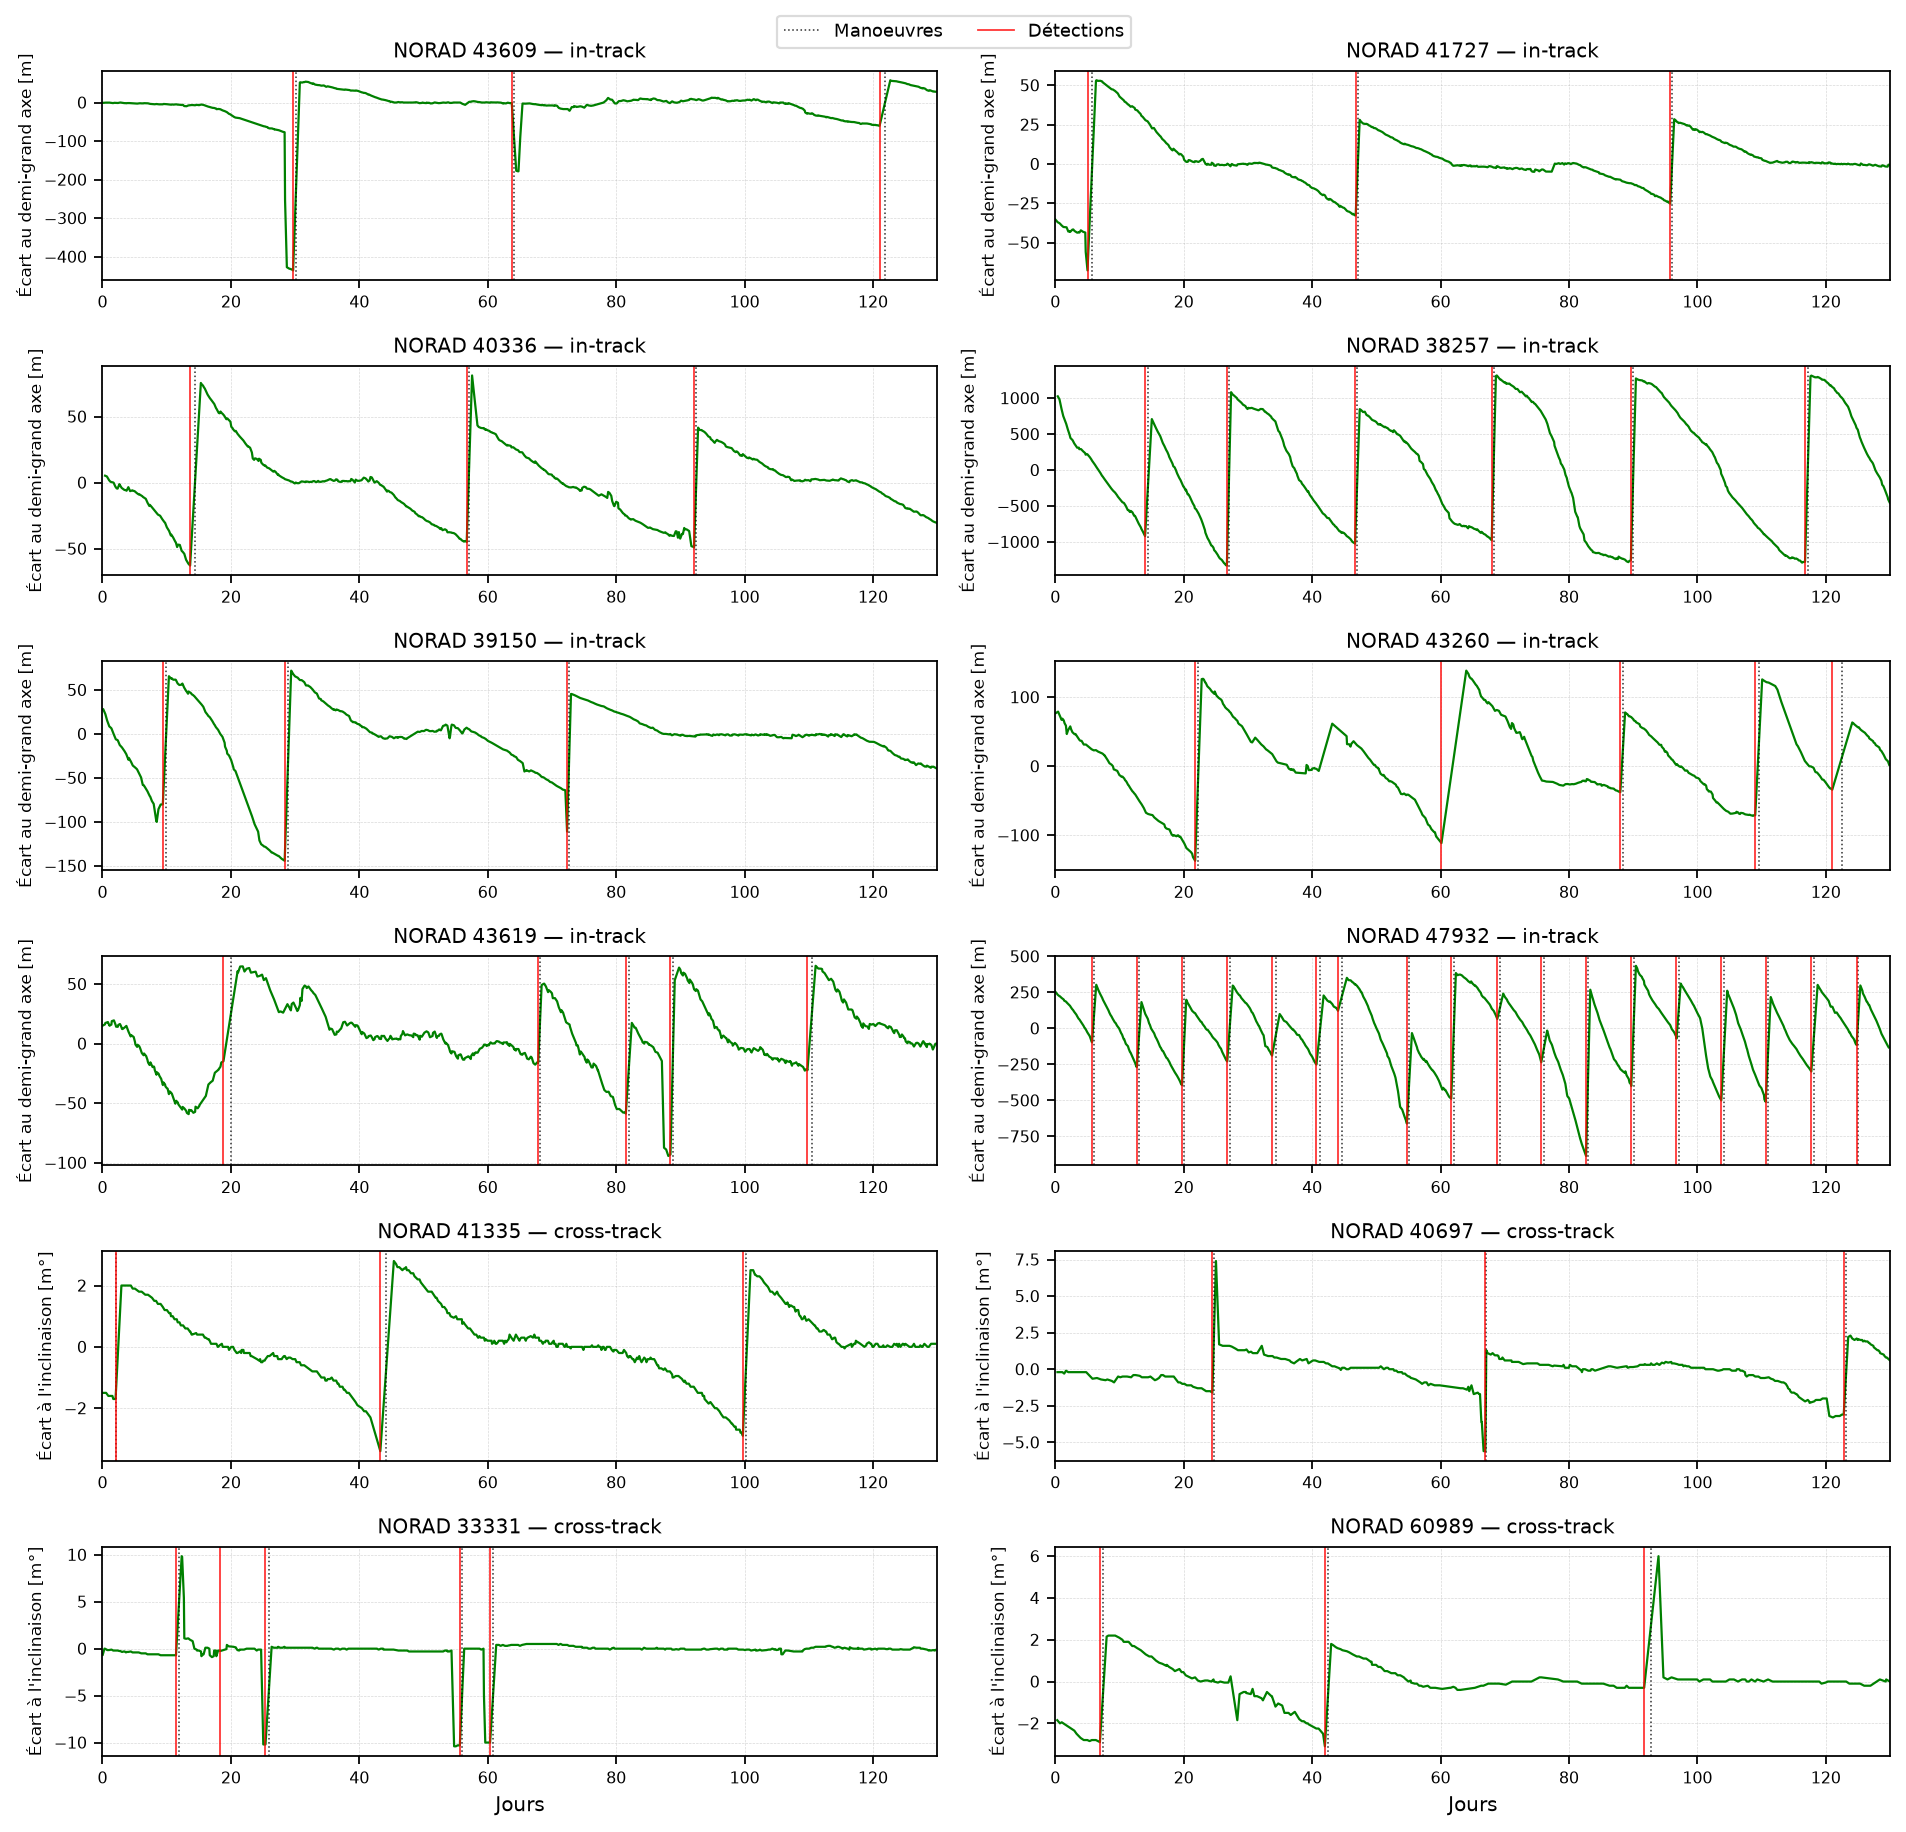
\includegraphics[width=\textwidth]{figures/stat_detections_sso.png}
\end{figure}

\begin{figure}[htbp]
\centering
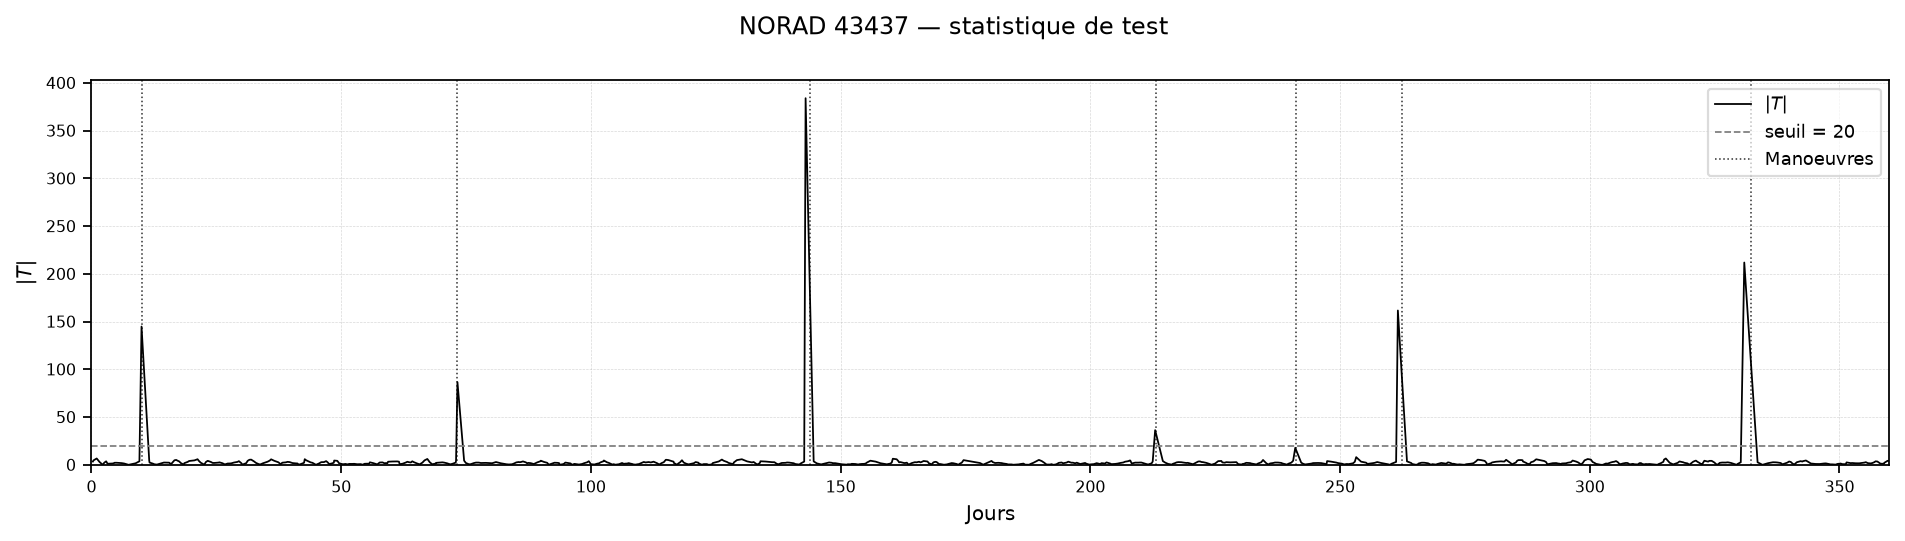
\includegraphics[width=\textwidth]{figures/stat_tstat.png}
\end{figure}

\end{document}
 